\chapter{Determinant of Infinite Matrices}

This chapter begins by thoroughly exploring the determinants of finite matrices, delving into their properties and applications. Emphasis is placed on how determinants are utilized in solving systems of linear equations within the finite matrix framework. The subsequent section extends this analysis to infinite matrices, examining the conditions that govern their determinants. Special attention is given to the complexities introduced by matrices of infinite dimension. The chapter concludes by applying determinants to resolve systems of linear equations involving infinite matrices. Overall, the chapter aims to provide a comprehensive understanding of both finite and infinite matrix determinants and their practical implications in the solution of linear systems. Here, we follow Matysiak et al.~\cite{amgopaper} for most of the defintions and results.

\section{Determinant of a finite matrix} 

For every square matrix $A = [a_{ij}]$, $1\leq i,j\leq n$, the \textbf{determinant} is a scalar value associated to $A$ that is a real or complex number, and it is denoted by $\det(A)$ or $|A|$. For $n = 1$, we assume $\det(A) = a_{11}$ and for $n\geq 2$, we define $\det(A)$ recursively, as follows:

For some fixed $i$,
\[
  \det(A) = \sum_{j=1}^{n} a_{ij} \cdot C_{ij}
\]

For some fixed $j$,
\[
  \det(A) = \sum_{i=1}^{n} a_{ij} \cdot C_{ij}
\]

where $C_{ij}$ is the cofactor of the element $a_{ij}$, $1\leq i,j\leq n$. Recall that the cofactor of an element of a matrix $A$ depends on the determinant of a lower order submatrix of $A$. In particular, for $n = 2$, we have 
\[
\det(A) = a_{11}C_{22}+a_{12}C_{21} = a_{11}a_{22}-a_{12}a_{21}.
\]


Consider the matrix $A$ as follows:

\[
A = \begin{bmatrix}
    a_{11} & a_{12} & \cdots & a_{1n} \\
    a_{21} & a_{22} & \cdots & a_{2n} \\
    \vdots & \vdots & \ddots & \vdots \\
    a_{n1} & a_{n2} & \cdots & a_{nn} \\
\end{bmatrix}
\]

Fix $i=1$. Then we find $\det(A)$ as follows:

\[
 \det(A) = a_{11} C_{11} + a_{12}C_{12} + \cdots + a_{1n}C_{1n}
\]

where
\[
\begin{aligned}
    C_{11} &= (-1)^{1+1} \begin{vmatrix} a_{22} & \cdots & a_{2n} \\ \vdots & \ddots & \vdots \\ a_{n2} & \cdots & a_{nn} \end{vmatrix}, \\\\
    C_{12} &= (-1)^{1+2} \begin{vmatrix} a_{21} & \cdots & a_{2n} \\ \vdots & \ddots & \vdots \\ a_{n1} & \cdots & a_{nn} \end{vmatrix},\\
    & \vdots \\
    C_{1n} &= (-1)^{1+n} \begin{vmatrix} a_{21} & \cdots & a_{n-1,n-1} \\ \vdots & \ddots & \vdots \\ a_{n1} & \cdots & a_{n,n-1} \end{vmatrix}.
\end{aligned}
\]




\vspace{30pt}
\section{Determinant of an infinite matrix}
A square matrix of infinite dimension is an infinite matrix in which the number of rows is equal to the number of columns. Let $M_n(R)$, $n\in \mathbb{N} \cup \{\infty\}$, denote the set of all square matrices of dimension $n$ with coefficients from any integral domain $R$ such that all the rows and columns of a matrix are convergent series.

A primary reason for choosing $n$ as an extended natural number, that is, $n\in\mathbb{N} \cup \{\infty\}$, is that upper and lower bounds of the extended natural numbers always exist~\cite{shivakumar1972diagonally}. Note that, $\infty$ is the largest element and $0$ is the smallest element in extended natural numbers. Also, every subset of extended natural numbers has the supremum and infimum. 

%Note also that, $M_n(R)$, $n\in \mathbb{N} \cup \{\infty\}$ is a ring. We check that $\{A \in M_n(\mathbb{Z}) : \det A \in \{-1, 1\}\}$ and $\{A \in M_n(\mathbb{Z}) : \det A = 1\}$ are multiplicative groups.

\medskip

The following result gives us a way to compute the determinant of an infinite dimensional square matrix.

\begin{theorem}~\cite{amgopaper}\label{deteminant_of_an_infinite_matrix}
Let $A_{n}$, where $n\in \mathbb{N}\cup \{\infty\}$, be a square matrix such that $\operatorname{tr}(\log A) = \sum_{k=1}^{\infty} (-1)^{k+1}\operatorname{tr}(\frac{(A-I)^k}{k})$ is a convergent series. Then $\det(A)$ is determined as follows:
\[\det(A) = \exp(\operatorname{tr}(\log A))\]
\end{theorem}


The following two examples illustrate the above result in the case of finite square matrices. 

Here, we use the MATLAB code Source Code~\ref{sourcecode-determinant} (Algorithm~\ref{alg-determinant-approximation}) to evaluate the terms of the logarithmic series involved in the aforesaid formula. \newline


\begin{example}
    Let
\[
A = \begin{bmatrix}
    0.8763 & 0.7373 & 0.2400 \\
    0.3106 & 1.2792 & 0.1884 \\
    0.2902 & 0.1537 & 0.1851
\end{bmatrix}.
\]
\newline
From Example~\ref{1.7.}, we have

$$\log(A)=
\begin{bmatrix}
   -0.3637 & 0.7554 & 0.4744 \\
    0.2523 & 0.1515 & 0.3026 \\
    0.7760 & -0.0110 & -2.0666
\end{bmatrix}
.$$

Then
\[\operatorname{tr}(\log A) = -2.2788\]
and hence 
\[\det A = \exp(\operatorname{tr}(\log A)) = 0.1024008543.\]

The approximated determinant of $A$ after $157$ iterations is $0.1024008544$.

The graph in Figure~\ref{graph-appdet-01} illustrates a rapid reduction in determinant error with increasing iterations, where the determinant error represents the disparity between the true and algorithmically estimated determinants of a matrix. Plotted on a logarithmic scale, each unit on the $y$-axis signifies a ten-fold change in determinant error. Notably, the graph signifies swift convergence of the algorithm, attaining a minimal error level around the $157$th iteration.

\begin{center}
    \begin{figure}[h] 
        \centering
        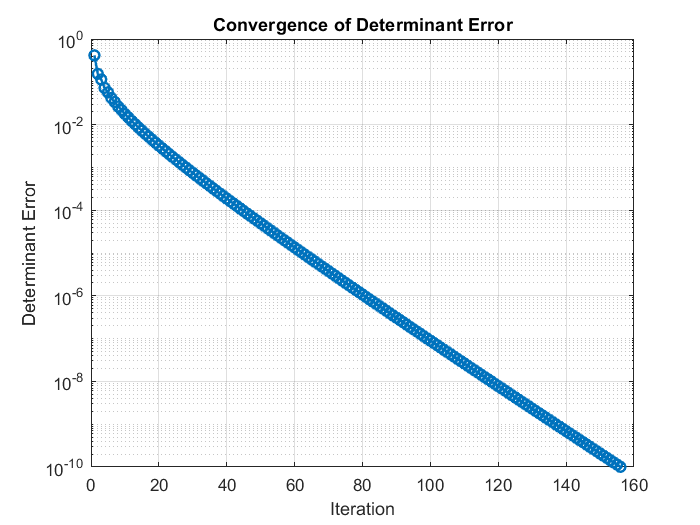
\includegraphics[width=0.8\linewidth]{Figures/determinant_error_plot_1.png}
        \caption{Convergence of determinant error over iterations (Case 1)}
        \label{graph-appdet-01}
    \end{figure}
\end{center}
\end{example}
\begin{example}
Consider the following matrix $A$.
\[
A = \begin{bmatrix}
    1.0000 & 0.0050 & 0.0050 & 0 & 0 & 0 & 0.0000 \\
    0.0100 & 0.6000 & 0 & 0 & 0 & 0 & 0 \\
    0 & 0 & 0.7000 & 0 & 0 & 0 & 0 \\
    0 & 0.1200 & 0 & 0.8000 & 0.1000 & 0 & 0.0010 \\
    0.0010 & 0 & 0.1250 & 0 & 0.9000 & 0 & 0.0010 \\
    0 & 0 & 0 & 0 & 0 & 0.9500 & 0 \\
    0 & 0.3000 & 0.2500 & 0 & 0 & 0 & 0.9800 \\
\end{bmatrix}
\]

We find that $\|I-A\|=0.554479<1$. Thus $\log(A)$ exists.  By using series expansion, we have

\[ \log(A)=
\begin{bmatrix}
    0 & 0.0064 & 0.0059 & 0 & 0 & 0 & 0 \\
    0.0128 & -0.5109 & -0.0000 & 0 & 0 & 0 & -0 \\
    0 & 0 & -0.3567 & 0 & 0 & 0 & 0 \\
   -0.0010 & 0.1724 & -0.0100 & -0.2231 & 0.1178 & 0 & 0.0011 \\
    0.0011 & -0.0002 & 0.1569 & 0 & -0.1054 & 0 & 0.0011 \\
    0 & 0 & 0 & 0 & 0 & -0.0513 & 0 \\
   -0.0021 & 0.3873 & 0.3004 & 0 & 0 & 0 & -0.0202 \\
\end{bmatrix}.
\]

Then by the definition of the logarithm of a matrix, we have

\[
   \det(A)=\exp(\operatorname{tr}(\log(A)) =0.2815109532.
\]

We find that the exact (up to 10 decimal places) determinant of $A$ is \(0.2815109532\) which equals the calculated determinant of $A$. Thus, the approximated determinant is correct up to 10 decimal places. 
\end{example}

The graph in Figure~\ref{graph-appdet-02} shows how the determinant error decreases as the number of iterations increases. The determinant error is the difference between the actual determinant of a matrix and the estimated determinant using an algorithm. The graph is plotted on a logarithmic scale, which means that each unit on the $y$-axis represents a ten-fold change in the determinant error. The graph shows that the algorithm converges quickly, reaching a very small error after about $35$ iterations.
\begin{center}
    \begin{figure}[h]
        \centering
        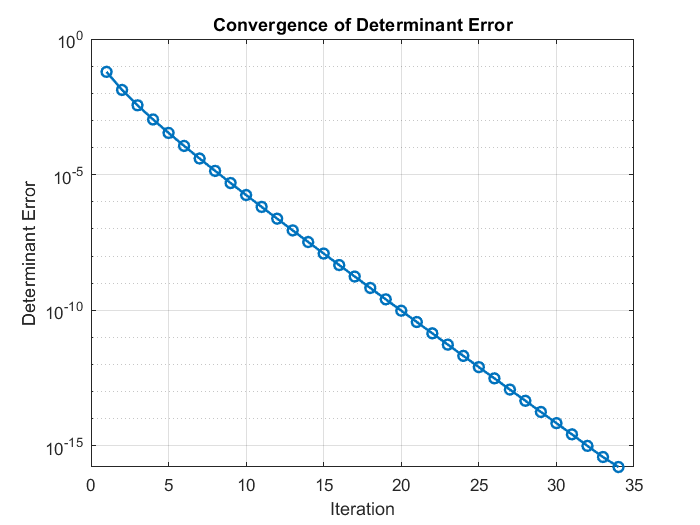
\includegraphics[width=0.8\linewidth]{Figures/det_error_higher_dim.png}
        \caption{Convergence of determinant error  over iterations (Case 2)}
        \label{graph-appdet-02}
    \end{figure}
\end{center}


% [The following section will go to another chapter regarding the application. So do not think about this.]



\medskip

\section{Determinant of matrix products}

To define the determinant of the product of infinite matrices we need the idea of equinumerous sets. A set $A$ is \textbf{equinumerous} to a set $B$, written $A \approx B$, if and only if there is a one-to-one function from $A$ onto $B$. For example, the sets $\mathbb{N}$ and $S=\{2, 4, 6, ...\}$ are equinumerous because the function $f: \mathbb{N}\to S$ defined as $f(n) = 2n$ is both one-one and onto.


\begin{definition}
  Consider the matrices $A_{m\times n}$ and $B_{n \times k}$, where $m,n,k\in \mathbb{N}\cup \{\infty\}$. For the matrix product $A_{m\times n}B_{n \times k}$, we get the following conclusions.
\begin{enumerate}
 \item[(a)] If $m = \infty$, $k = \infty$, then $AB = C_{\infty \times \infty}$.
 \item[(b)] If $n = \infty$, then $AB = C_{m \times k} = [c_{ij}]$, where $c_{ij} = \sum_{l=1}^{\infty} a_{il}b_{lj}$, $1 \leq i \leq m$, $1 \leq j \leq k$, are all convergent series.
 \item[(c)] If $A$ and $B$ are square matrices of infinite dimension then $AB = C$ holds.
 \item[(d)] If $A$ and $B$ are matrices of infinite dimension, and the number of rows in $A$ is equinumerous to the number of columns in $B$, then we find the product $AB$ only if rows of $A$ and columns of $B$ are convergent series.
\end{enumerate}
\end{definition}





The following result gives an important property regarding the determinant of the product of infinite matrices.  

\begin{proposition}~\cite{amgopaper}
 Let $A$ be an $m$-by-$n$ matrix, and let $B$ be an $n$-by- $m$ matrix, where $m, n \in \mathbb{N} \cup \{\infty\}$. Let $1 \leq j_1, j_2, \ldots, j_m \leq n$. Let $A_{j_1j_2\ldots j_m}$ denote the $m$-by-$m$ matrix consisting of columns $j_1, j_2, \ldots, j_m$ of $A$. Let $B_{j_1j_2\ldots j_m}$ denote the $m$-by-$m$ matrix consisting of rows $j_1, j_2, \ldots, j_m$ of $B$. Then
\[\det(AB) = \sum_{1 \leq j_1 < j_2 < \ldots < j_m \leq n} \det(A_{j_1j_2\ldots j_m}) \det(B_{j_1j_2\ldots j_m}).\]
\end{proposition}


\begin{proof}
First, we will show the proof in the finite version. Let $(k_1, k_2, \ldots, k_m)$ be an ordered $m$-tuple of integers. Let $\eta(k_1, k_2, \ldots, k_m)$ denote the sign of $(k_1, k_2, \ldots, k_m)$. Let $(l_1, l_2, \ldots, l_m)$ be the same as $(k_1, k_2, \ldots, k_m)$ except for $k_i$ and $k_j$ having been transposed. Then, from Transposition is of Odd Parity
\[\eta(l_1, l_2, \ldots, l_m) = -\eta(k_1, k_2, \ldots, k_m).\]
Let $(j_1, j_2, \ldots, j_m)$ be the same as $(k_1, k_2, \ldots, k_m)$ by arranging into non-decreasing order. That is $j_1 \leq j_2 \leq \ldots \leq j_m$. Then, it follows that
\[\det(B_{k_1\ldots k_m}) = \eta(k_1, k_2, \ldots, k_m) \det(B_{j_1\ldots j_m}).\]
Hence
\begin{align*}
    \det(AB) &= \sum_{1 \leq l_1, \ldots, l_m \leq m} \eta(l_1, \ldots, l_m) \left(\sum_{k=1}^n a_{1k}b_{k,l_1}\right) \ldots \left(\sum_{k=1}^n a_{mk}b_{k,l_m}\right) \\
    &= \sum_{1 \leq k_1, \ldots, k_m \leq n} \sum_{k=1}^n a_{1k} \ldots a_{mk} \sum_{1 \leq l_1, \ldots, l_m \leq m} \eta(l_1, \ldots, l_m) b_{k_1,l_1} \ldots b_{k_m,l_m} \\
    &= \sum_{1 \leq k_1, \ldots, k_m \leq n} \sum_{k=1}^n a_{1k} \ldots a_{mk} \det(B_{j_1\ldots j_m}) \\
    &= \sum_{1 \leq k_1, \ldots, k_m \leq n} \sum_{k=1}^n a_{1k} \ldots a_{mk} \det(B_{k_1\ldots k_m}) \\
    &= \sum_{1 \leq k_1, \ldots, k_m \leq n} a_{1k_1} \ldots a_{mk_m} \eta(k_1, \ldots, k_m) \det(B_{j_1\ldots j_m}) \\
    &= \sum_{1 \leq j_1 \leq j_2 \leq \ldots \leq j_m \leq n} \det(A_{j_1\ldots j_m}) \det(B_{j_1\ldots j_m}).
\end{align*}

If two $j$'s are equal then
\[\det(A_{j_1\ldots j_m}) = 0.\]

For infinite matrices, we put $\infty$-tuple of the form $(k_1, k_2, k_3, \ldots)$ and put $1 \leq j_1, j_2, j_3, \ldots < n = \infty$.
\end{proof}
      

The following example illustrates the result obtained above in the case of finite dimensional matrices. 

\begin{example}

Consider the non-square matrices
\[
A = \begin{bmatrix} 1 & 2 & 3 \\ 4 & 5 & 6 \end{bmatrix} \quad\text{and}\quad
B = \begin{bmatrix} 7 & 8 \\ 9 & 10 \\ 11 & 12 \end{bmatrix}.
\]

According to the given proposition, consider all possible combinations of distinct indices $j_1 < j_2$ from the set $\{1, 2, 3\}$ to form submatrices $A_{j_1j_2}$ and $B_{j_1j_2}$. The determinant of the product $A_{j_1j_2}B_{j_1j_2}$ is then calculated, and the sum of all these determinants should be equal to $\det(AB)$.

Let us consider $j_1 = 1$ and $j_2 = 2$. Then we have
\[
A_{12} = \begin{bmatrix} 1 & 2 \\ 4 & 5 \end{bmatrix} \quad\text{and}\quad B_{12} = \begin{bmatrix} 7 &  8 \\ 9 & 10 \end{bmatrix}.
\]

Then
\[
\det(A_{12}) = -3 \quad\text{and}\quad \det(B_{12}) = -2.
\]

Again for $j_1=1$ and $j_2=3$, we have
\[ A_{13} = \begin{bmatrix} 1 & 3 \\ 4 & 6 \end{bmatrix} \quad\text{and}\quad B_{13} = \begin{bmatrix} 7  & 8 \\ 11 & 12 \end{bmatrix}. \]

Then
\[ \det(A_{13}) = -6 \quad\text{and}\quad \det(B_{13}) = -4. \]


Again for \(j_1 = 2\) and \(j_2 = 3\), we have
\[ A_{23} = \begin{bmatrix} 2 & 3 \\ 5 & 6 \end{bmatrix} \quad\text{and}\quad B_{23} = \begin{bmatrix} 9 & 10 \\ 11 & 12 \end{bmatrix}. \]

Then
\[ \det(A_{23}) = -3 \quad\text{and}\quad \det(B_{23}) = -2. \]

Now by summing up all the determinants, we have 
\[
\det(AB) = \sum_{1 \leq j_1 < j_2 \leq 3} \det(A_{j_1j_2}) \det(B_{j_1j_2})
\]
\[
= (-3) \cdot (-2) + (-6) \cdot (-4) + (-3) \cdot (-2) = 36.
\]


On the other hand, we calculate $AB$ as follows:
\[
AB = \begin{bmatrix} 1 \cdot 7 + 2 \cdot 9 + 3 \cdot 11 & 1 \cdot 8 + 2 \cdot 10 + 3 \cdot 12 \\ 4 \cdot 7 + 5 \cdot 9 + 6 \cdot 11 & 4 \cdot 8 + 5 \cdot 10 + 6 \cdot 12 \end{bmatrix}
= \begin{bmatrix} 58 & 64 \\ 139 & 154 \end{bmatrix}
\]
Then $\det(AB)=36$.

So, the final result of \(\det(AB)\) is \(36\), and it matches the sum of the determinants of the submatrices as predicted by the proposition. The steps include calculating the determinants for all valid combinations of indices and summing them up.

\end{example}






\section{Applications of determinant}

Let $A$ be an $m$-by-$n$ matrix over an arbitrary field $\mathbb{F}$ $(m, n \in \mathbb{N} \cup \{\infty\})$. There is an associated linear mapping $f: \mathbb{F}^n \to \mathbb{F}^m$ defined by $f(x) = Ax$. The rank of $A$ is the dimension of the image $f$. This definition has the advantage that it can be applied to any linear map without the need for a specific matrix.
Consider the system of equations
\[
\begin{rcases}
    \begin{aligned}
        &a_{11}x_1 + a_{12}x_2 + a_{13}x_3 + \dots  = b_1 \\
        &a_{21}x_1 + a_{22}x_2 + a_{23}x_3 + \dots  = b_2 \\
        &a_{31}x_1 + a_{32}x_2 + a_{33}x_3 + \dots = b_3 \\
        & \hspace{2.75cm}\vdots\\
    \end{aligned}
\end{rcases}
\]
denoted as $AX = B$. By Cramer's system, we mean a system in which the number of equations is equal to the number of unknowns. Then, Cramer's theorem states that in the finite case, the system has a unique solution provided we have $n$ equations. Hence, individual values for the unknowns are given by
\[
x_i = \frac{A_{x_i}}{\operatorname{det } (A)},
\]
for $i = 1, 2, \dots$, where $A_{x_i}$ is the determinant of the matrix obtained by replacing the $i^{th}$ column of $A$ by the column vector $B$. If $\operatorname{tr } A_{x_i}$ and $\operatorname{tr } A$ are convergent series, then Cramer's formula holds for the infinite case.

On the other hand, for a system of equations $AX = B$ where $A, X, B$ can have an infinite dimension, it implies $X = A^{-1}B$.
\[
A = \begin{bmatrix}
    a_{11} & a_{12} & a_{13} & \cdots &  \\
    a_{21} & a_{12} & a_{23} & \cdots &  \\
    a_{31} & a_{32} & a_{33} & \cdots &  \\
    \vdots & \vdots & \vdots & \ddots &  
 \end{bmatrix}
\]
\[
B = \begin{bmatrix}
    b_{11} \\
    b_{21} \\
    b_{31} \\
    \vdots  \\
\end{bmatrix}
\]


At first, we find the determinant of the coefficient matrix of $A$ as follows:
\[
{\operatorname{det } (A)} = \begin{vmatrix}
    a_{11} & a_{12} & a_{13} & \cdots &  \\
    a_{21} & a_{12} & a_{23} & \cdots &  \\
    a_{31} & a_{32} & a_{33} & \cdots &  \\
    \vdots & \vdots & \vdots & \ddots &  \\
\end{vmatrix}
\]

Then we find the determinant $A_{x_1}$ as follows:
\[
     A_{x_1} = \begin{vmatrix}
    b_1 & a_{12} & a_{13} & \cdots &  \\
    b_2 & a_{22} & a_{23} & \cdots &  \\
    b_3 & a_{32} & a_{33} & \cdots &  \\
    \vdots & \vdots & \vdots & \ddots &  \\
\end{vmatrix}
\]

Then we have 
\[
x_1 = \frac{ A_{x_1}}{\operatorname{det } (A)}.
\]

Similarly, we find
\[
     A_{x_2} = \begin{vmatrix}
    a_{11} & b_1 & a_{13} & \cdots &  \\
    a_{21} & b_2 & a_{23} & \cdots &  \\
    a_{31} & b_3 & a_{33} & \cdots &  \\
    \vdots & \vdots & \vdots & \ddots &  \\
\end{vmatrix}.
\]

which gives
\[
x_2 = \frac{ A_{x_2}}{\operatorname{det } (A)}
\]

and we find
\[
    A_{x_3} = \begin{vmatrix}
    a_{11} & a_{12} & b_1 & \cdots &  \\
    a_{21} & a_{22} & b_2 & \cdots &  \\
    a_{31} & a_{32} & b_3 & \cdots &  \\
    \vdots & \vdots & \vdots & \ddots &  \\
\end{vmatrix}
\]

which gives 
\[
x_3 = \frac{ A_{x_3}}{\operatorname{det } (A)}.
\]

Similarly for all $i=1, 2, 3, \ldots$, we find
\[
      A_{x_i} = \begin{vmatrix}
    a_{11} & a_{12} & \cdots & \cdots & b_1 & \cdots &  \\
    a_{21} & a_{22} & \cdots & \cdots & b_2 & \cdots &  \\
    a_{31} & a_{32} & \cdots & \cdots & b_3 & \cdots &  \\
    \vdots & \vdots & \vdots & \vdots & \vdots & \ddots & \\
\end{vmatrix}.
\]

These give the value of $i^{th}$ variable $x_i$ for all $i=1, 2, 3, \ldots$ as follows:
\[
x_i = \frac{ A_{x_i}}{\operatorname{det } (A)}.
\]
